% Copy of docs/manuscript/elsevier/supplement.tex (generated from docs/manuscript/ieee/supplement.tex); only the title was changed to match final_v3/main.tex.
\documentclass[preprint,12pt]{elsarticle}

\usepackage[utf8]{inputenc}
\usepackage[T1]{fontenc}
\usepackage{amsmath,amssymb}
\usepackage{graphicx}
\usepackage{booktabs}
\usepackage{multirow}
\usepackage{array}
\usepackage{adjustbox}
\usepackage{longtable}
\emergencystretch=1.5em
\usepackage{url}
\usepackage{xcolor}
\usepackage[hidelinks]{hyperref}

% Content that is already written but must be confirmed or completed by the authors carries a
% visible marker. REMOVE EVERY \pending{...} BEFORE SENDING (grep -n "pending{" main.tex).
\newcommand{\pending}[1]{\textcolor{red}{\textbf{[PENDING: #1]}}}

\graphicspath{{../figures/}}
\journal{Simulation Modelling Practice and Theory}

\renewcommand{\thesection}{S-\Roman{section}}
\renewcommand{\thetable}{S-\Roman{table}}
\renewcommand{\thefigure}{S-\arabic{figure}}

\begin{document}

\begin{frontmatter}

\title{Supplementary material: When Proximity Is Not Interception: Auditing Capture Endpoints and Predictive Lane Blocking for Vehicle Pursuit in Microscopic Urban Traffic Simulation}

\author[1]{Andrei Noguera Gil\corref{cor1}}
\ead{0187940@up.edu.mx}
\author[1]{Felix Martinez-Rios}
\ead{fmartin@up.edu.mx}
\author[2]{Edgar Avalos-Gauna}
\ead{ea37@rice.edu}
\cortext[cor1]{Corresponding author.}

\affiliation[1]{organization={Universidad Panamericana, Facultad de Ingenier\'{\i}a},
            addressline={Augusto Rodin 498},
            city={Ciudad de M\'exico},
            postcode={03920},
            country={M\'exico}}

\affiliation[2]{organization={Rice University},
            addressline={6100 Main Street},
            city={Houston},
            state={Texas},
            postcode={77005-1827},
            country={United States}}

\end{frontmatter}



\noindent This supplement gives the audit details, the full tables and the secondary analyses behind the main article.
Section and table numbers carry the prefix ``S''. Terms and abbreviations are those of the article: operational
capture (OC), predictive lane blocking (PLB), the TRAINING, DEVELOPMENT and TEST cities, and the second held-out
set, HELD-OUT~B. The code, the analyses and the data figures reported here were produced with the AI assistance that
the article describes in its section on protocol and statistics, under the same safeguards.

% =====================================================================================================
\section{Persistence Audit of Operational Captures}\label{sec:s-hold}

Table~\ref{tab:s-persistence} reports the hold audit. In the original audit, 188 of 1\,433 replays had less than
60\,s of follow-up because the episode horizon ended. A versioned replay extended these to 60\,s. A second replay
verified that each extension reproduced the original capture (same time and finisher) and that the natural and held
replays agreed in position and speed at the moment the pursuers were held (188/188). With complete follow-up, no escape
was observed in the 1\,433 audited captures. They come from 176 scenario--evader families in seven cities and share
families across methods, team sizes and seeds, so we report the count rather than an independence-based bound.
Captures next to a red signal or a free adjacent lane are rare.

\begin{table}[!h]
\centering
\caption{Hold audit of OC captures (60\,s complete follow-up for all after a versioned replay of 188 censored cases).}
\label{tab:s-persistence}
\begin{adjustbox}{max width=\textwidth}
\begin{tabular}{@{}lccc@{}}
\toprule
& PLB & Ambush & Pursuit \\
\midrule
Captures audited & 562 & 480 & 391 \\
Censored originally ($<60$\,s) & 82 & 64 & 42 \\
\textbf{Escape, pursuers held} & \textbf{0} & \textbf{0} & \textbf{0} \\
Red/yellow signal $\le$40\,m & 2.0\% & 2.7\% & 3.1\% \\
Free adjacent lane & 1.6\% & 1.5\% & 2.0\% \\
Released if re-planning & 8.4\% & 14.4\% & 12.8\% \\
\bottomrule
\end{tabular}
\end{adjustbox}
\end{table}

\emph{Capture instants re-verified.} The instant at which the pursuers were held came from a helper that kept a
pursuer's run of valid frames open when that pursuer was absent from a frame, so that two separate fragments could be
joined into one witness. A fifth audit showed this on a constructed trace. The traces of the audit had not been
stored, so all 1\,433 captures were replayed, and each instant was recomputed with a corrected extractor, which ends
a run when the pursuer or the evader is absent or a value is invalid, and with the judge applied to each pursuer
alone. Every replay reproduced the sealed instant and finisher, and the three computations agree in all 1\,433
captures. No hold audit therefore started from a wrong instant, and the results above stand. The condition that
breaks the earlier helper does occur in this simulator: in 4 of the 1\,433 traces a pursuer is absent for 0.4\,s or
2.5\,s and then present again. In all four it is not the pursuer that completes the capture. No collision occurred
in these episodes.

\emph{Active-escape probe.} The hold audit was repeated with a probe that, from the moment of capture, requests every
second a change to an adjacent lane with an onward link and a reroute through it, with safety checks on. Among the
1\,433 reproduced captures, 15 escapes were observed, from 3 of 176 families. Lane-change requests were recorded in
115 episodes, which include all 15 escapes. In 1\,316 episodes only reroute requests were recorded, and no escape was
observed. Two episodes produced only control errors and are inconclusive for this test. The absence of a recorded
lane-change request is not proof that no adjacent exit existed: the probe did not take an independent inventory of
lanes at capture, and it did not verify that a requested manoeuvre was executed. Reversing and mid-edge U-turns were
not evaluated. An earlier version of this analysis presented the request groups as geometric groups; that reading is
withdrawn.

% =====================================================================================================
\section{Capture Events in a Published Environment}\label{sec:s-published}

\emph{Source.} We used the official repository of DGMARL-MVP \cite{li2023dgmarl}
(\url{https://github.com/BUPT-ANTlab/DGMARL-MVP}, commit \texttt{62bd72e2}). Before running it we reviewed the code.
The environment, which is the only part we executed, opens no network connection, evaluates no external input and
deletes no file; it starts SUMO. Compiled files shipped with the repository were deleted without being run. The
repository has no licence file, so we cite and evaluate it and do not redistribute it. Each worker ran a
byte-identical copy of the source files (their hashes are stored with the results). Nothing in the code was edited. The only values set
from outside are ones the code exposes: the path of the SUMO binary (undefined on our platform in the release), the
TraCI port and the scenario name.

\emph{What the released code does.} A capture is declared when the distance between the positions of a pursuer and an
evader is below 5\,m. In SUMO these positions are the front-bumper points. The evader is then removed from the
simulation, and the episode succeeds when all evaders have been removed within 800 steps of 1\,s. Evaders turn at
random at each junction. Pursuers choose left, straight or right at the next junction; they have no action to stop or
to wait. The network is a grid of 16 junctions with one 3.2\,m lane per direction, 5\,m vehicles and 200 background
vehicles. A follower in the same lane is at least one vehicle length plus a gap behind its leader's front bumper, so
the rule cannot be met by following; we recorded this as a prediction before the run.

\emph{Released versus reported configuration.} The article does not state the capture distance; the code does. The
release also differs from the reported settings: the learning rates are $10^{-12}$ in the release and $10^{-4}$ in the
article, the lane speed limit is 13.9\,m/s against a reported maximum of 20\,m/s, and no trained weights are provided.
We used SUMO 1.21; the authors' version is not stated. We therefore audit the released environment and do not
reproduce the article's numbers.

\emph{Design} (registered before the run). Two scenarios as released: four pursuers and two evaders (300 episode
seeds) and seven pursuers and four evaders (100 seeds). Two teams, with the same seeds:
\begin{itemize}
\item a \emph{null} team, in which every pursuer turns uniformly at random;
\item a \emph{chaser} team, in which every pursuer takes the turn whose next road is closest, by shortest path in the
environment's own road graph, to the road of the nearest remaining evader.
\end{itemize}
Each episode ran in two modes. In the \emph{published} mode the environment is unmodified, and an observer reads the
state of the capturing pair before the evader is removed. In the \emph{follow-up} mode the episode is identical until
the first capture; the evader is then left in the simulation, and it is followed for 30\,s while the pursuers keep
their policy and keep it as a target. All 1\,600 episodes completed. Eight episodes run beforehand as an execution
check were reproduced identically. In 12 of the 577 first captures the episode horizon ended before the 30\,s had
passed. A versioned addendum re-ran those 12 with the horizon extended; each reproduced the same first event, so the
follow-up rows of Table~\ref{tab:s-published} cover all 577 first captures. The same addendum re-ran the 800
unmodified episodes to measure the stop analogue of the last row with a duration in simulation time; all 800
reproduced the original capture events.

\begin{table}[!h]
\centering
\caption{Capture events in the official DGMARL-MVP environment, released configuration. P4--E2: four pursuers and two
evaders; P7--E4: seven and four. Episode-level 95\% bootstrap intervals.}
\label{tab:s-published}
\small
\setlength{\tabcolsep}{5pt}
\begin{adjustbox}{max width=\textwidth}
\begin{tabular}{@{}lcccc@{}}
\toprule
& \multicolumn{2}{c}{P4--E2} & \multicolumn{2}{c}{P7--E4} \\
& Null & Chaser & Null & Chaser \\
\midrule
Episodes & 300 & 300 & 100 & 100 \\
Published success & 42.7\% [37.3, 48.3] & 4.0\% [2.0, 6.3] & 39.0\% [30.0, 48.0] & 2.0\% [0.0, 5.0] \\
At least one capture & 90.0\% & 42.3\% & 100.0\% & 80.0\% \\
Share of evaders captured & 66.3\% & 23.2\% & 81.2\% & 34.2\% \\
Mean steps & 673 & 789 & 687 & 798 \\
Capture events & 398 & 139 & 325 & 137 \\
\quad same lane & 0 & 0 & 0 & 0 \\
\quad opposite directions & 82.9\% & 59.7\% & 82.5\% & 70.8\% \\
\quad inside a junction & 17.1\% & 40.3\% & 17.5\% & 29.2\% \\
\quad headings differ by $\ge150^\circ$ & 93.7\% & 92.1\% & 91.4\% & 94.9\% \\
\quad evader faster than 1\,m/s & 75.6\% & 90.6\% & 70.5\% & 89.0\% \\
\quad median front-to-front distance & 3.6\,m & 3.7\,m & 3.7\,m & 3.7\,m \\
\midrule
First captures followed for 30\,s & 270 & 127 & 100 & 80 \\
\quad identical to the unmodified run & 270/270 & 127/127 & 100/100 & 80/80 \\
\quad $+1$\,s: within 5\,m of its captor & 12.2\% & 23.6\% & 9.0\% & 17.5\% \\
\quad $+5$\,s: within 5\,m of its captor & 0 of 270 & 0 of 127 & 0 of 100 & 0 of 80 \\
\quad $+10$\,s: evader faster than 1\,m/s & 75.2\% & 91.3\% & 67.0\% & 85.0\% \\
\quad $+10$\,s: over 50\,m from every pursuer & 94.8\% [92.2, 97.4] & 92.9\% [88.2, 96.9] & 95.0\% [90.0, 99.0] & 92.5\% [86.2, 97.5] \\
\quad $+30$\,s: median distance to its captor & 439\,m & 423\,m & 449\,m & 423\,m \\
\midrule
Evaders stopped $\ge$2\,s behind one stopped pursuer & 3.8\% & 2.5\% & 4.0\% & 3.2\% \\
\bottomrule
\end{tabular}
\end{adjustbox}
\end{table}

\emph{Reading.} Table~\ref{tab:s-published} shows the same pattern in both scenarios. No capture event joined two
vehicles in the same lane; more than nine in ten joined vehicles with nearly opposite headings, at a median distance
close to the 3.2\,m that separates the two lanes of a road. In the follow-up mode, the first capture was the same
event as in the unmodified run in every episode. One second later, most evaders were already more than 5\,m from the
vehicle that had captured them; five seconds later, all 577 were. The share of evaders that were ever stopped for at
least 2\,s behind one and the same stopped pursuer, which is the closest analogue of an operational stop that this
action space allows, was 2.5--4.0\%, and arose from ordinary queues.

\emph{Scope.} The article reports success rates of 0.77--0.91 (P4--E2) and 0.73--0.81 (P7--E4) for four learned
methods, over 100 test episodes \cite{li2023dgmarl}. Our null team reaches about half of those values without
pursuing, and a team that chases reaches almost none. Because of the configuration differences listed above, and
because we did not train the published learner, this is not a reproduction and it is not evidence about that learner.
It is evidence about the endpoint: in this environment the published rule is met by crossing the evader's path.

\emph{A second environment: PEPCRL-MVP.} The audit was repeated on the official repository of PEPCRL-MVP
\cite{li2024pepcrl} (commit \texttt{ac8ca695}, run unmodified with SUMO 1.21). Its release contains a real map of 53
two-way roads with one lane per direction, about 300 background vehicles, and three scenarios: 6 pursuers and 3
evaders, 7 and 4, and 8 and 5. The capture rule is that of the first environment, a distance below 5\,m between
vehicle positions with removal of the evader, over 800 steps. The design is the one above, with a simulation-time
stop analogue and complete follow-up from the start; 150 seeds per scenario, team and mode, 1\,800 episodes. One
prediction was registered before the run: with 5\,m vehicles, front-bumper positions and one lane per direction, no
capture event would join two vehicles in the same lane.

\begin{table}[!h]
\centering
\caption{Capture events in the official PEPCRL-MVP environment (released real map, 150 episodes per team, scenario
and mode). Success uses completed episodes of the unmodified mode, with episode-level 95\% bootstrap intervals;
capture events include those recorded before an abort; follow-up rows come from the separate follow-up mode. An
episode that the unmodified environment aborted is not replaced.}
\label{tab:s-pepcrl}
\small
\setlength{\tabcolsep}{3pt}
\begin{adjustbox}{max width=\textwidth}
\begin{tabular}{@{}lcccccc@{}}
\toprule
& \multicolumn{2}{c}{6 pursuers, 3 evaders} & \multicolumn{2}{c}{7 pursuers, 4 evaders} & \multicolumn{2}{c}{8 pursuers, 5 evaders} \\
& Null & Chaser & Null & Chaser & Null & Chaser \\
\midrule
Episodes completed, of 150 & 150 & 142 & 149 & 149 & 150 & 144 \\
Published success & 31.3\% & 2.8\% & 59.1\% & 10.7\% & 58.7\% & 9.7\% \\
\quad 95\% interval & [24.0, 38.7] & [0.7, 5.6] & [51.0, 67.1] & [6.0, 16.1] & [50.7, 66.7] & [4.9, 14.6] \\
Capture events & 295 & 138 & 520 & 314 & 669 & 444 \\
\quad of which before an abort & 0 & 8 & 2 & 1 & 0 & 11 \\
\quad same lane & 0 & 0 & 0 & 0 & 0 & 0 \\
\quad opposite directions & 78.3\% & 82.6\% & 76.3\% & 79.0\% & 79.4\% & 75.7\% \\
\quad inside a junction & 21.7\% & 16.7\% & 23.6\% & 21.0\% & 20.6\% & 24.3\% \\
\quad evader faster than 1\,m/s & 61.4\% & 85.5\% & 67.1\% & 79.9\% & 71.0\% & 79.5\% \\
\midrule
First captures followed for 30\,s & 142 & 96 & 150 & 143 & 150 & 146 \\
\quad $+5$\,s: within 5\,m of its captor & 1.4\% & 0.0\% & 0.0\% & 0.0\% & 0.0\% & 0.0\% \\
\quad $+10$\,s: over 50\,m from every pursuer & 79.6\% & 62.5\% & 83.3\% & 69.2\% & 82.7\% & 73.3\% \\
Evaders stopped $\ge$2\,s behind one stopped pursuer & 4.4\% & 6.1\% & 6.2\% & 8.9\% & 5.3\% & 11.2\% \\
\bottomrule
\end{tabular}
\end{adjustbox}
\end{table}

\emph{Denominators.} Each scenario and team was run with the same 150 seeds in two modes, which are separate
simulations: 900 episodes with the unmodified dynamics (\emph{published} mode) and 900 in \emph{follow-up} mode. Of
the 1\,800 scheduled episodes, 1\,781 completed: 884 in published mode and 897 in follow-up mode. Nineteen aborted
inside the released environment, which has no branch for a pursuer that SUMO is teleporting or for an evader that
has left; at most 8 of 150 in one cell, below the limit of 20\% registered for interpreting a cell. Three kinds of
figure therefore have three denominators. Success rates use the completed episodes of the published mode (the first
row of Table~\ref{tab:s-pepcrl}). The capture events are all the events of the published mode, 2\,380: 2\,358 from
completed episodes and 22 recorded in 13 episodes before the environment aborted them. An event before an abort is
a valid event of the unmodified dynamics, and keeping it was fixed before the run; the table gives their number per
cell. The follow-up figures use the first captures of the follow-up mode.

The prediction held: none of the 2\,380 capture events joined two vehicles in the same lane, neither among the
2\,358 of completed episodes nor among the 22 recorded before an abort (Table~\ref{tab:s-pepcrl}). The null team met the published criterion in 31--59\% of
episodes and the chaser in 3--11\%. The first capture was the same event as in the unmodified run in 814 of 814
checked episodes; all 827 first captures have 30\,s of follow-up, and 2 of the 827 evaders were within 5\,m of their
captor after 5\,s. After 10\,s, 76\% were more than 50\,m from every pursuer, fewer than on the grid: the map is
smaller and the teams larger. The article reports success rates of 0.68, 0.62 and 0.56 for its method in the three
scenarios, and 0.27--0.62 for eight baselines, over 100 tests; in the two larger scenarios the null team is at the
level of the proposed method. As before, the released configuration may differ from the reported one, a later SUMO
version was used and the learner was not trained, so this is evidence about the endpoint and not about the learner.
The two audited environments come from one research group and share code. The second adds a real map and a journal
article; it does not add an independent group.

% =====================================================================================================
\section{Other Controllers and Full Tables}\label{sec:s-controllers}

\emph{Cut.} A further heuristic controller assigns distinct gates to the pursuers by urgency. On real cities, pursuit
and cut perform alike. Against the optimal evader, pursuit is better by 0.08--0.10. For pursuit and cut teams, the
excess over the independence reference is at most zero in all ten cells. On literature-like grids, cut beats pursuit
by $+0.29$ [0.19, 0.38].

\emph{Junction ambush.} The junction ambush beats pursuit by $+0.04$ to $+0.12$, but a full ambush was feasible in only
8--18\% of decision steps, which motivated pre-positioning.

\emph{Held-out evaluation.} Table~\ref{tab:s-test} is the full table of the single-shot evaluation, including the two
controllers of the first MAPPO study (A), which imitate PLB. They show no detected difference from it: KAN $-0.001$
[$-$0.040, 0.037] and MLP $-0.009$ [$-$0.048, 0.030]. No cell exceeds the independence reference.

\begin{table}[!h]
\centering
\caption{Single-shot evaluation on the four TEST cities with frozen methods. OC capture rates. 7\,200 team episodes
were scheduled for the five methods. 210 failed scenario placement, in 42 conditions failing identically for all five
methods, leaving 6\,990 completed. Single-pursuer and certificate-replay runs are reported separately.}
\label{tab:s-test}
\begin{adjustbox}{max width=\textwidth}
\begin{tabular}{@{}llccccc@{}}
\toprule
Evader & Team & PLB & Junction ambush & Pursuit & MAPPO-KAN (A) & MAPPO-MLP (A) \\
\midrule
\multirow{3}{*}{Random} & 3 & 0.299 & 0.175 & 0.162 & 0.299 & 0.305 \\
& 5 & 0.351 & 0.260 & 0.221 & 0.396 & 0.377 \\
& 7 & 0.370 & 0.292 & 0.292 & 0.448 & 0.468 \\
\midrule
\multirow{3}{*}{Avoidant} & 3 & 0.297 & 0.203 & 0.127 & 0.259 & 0.241 \\
& 5 & 0.373 & 0.253 & 0.171 & 0.323 & 0.316 \\
& 7 & 0.367 & 0.266 & 0.215 & 0.329 & 0.304 \\
\midrule
\multirow{3}{*}{Optimal} & 3 & 0.253 & 0.156 & 0.130 & 0.247 & 0.234 \\
& 5 & 0.260 & 0.188 & 0.091 & 0.273 & 0.286 \\
& 7 & 0.364 & 0.260 & 0.143 & 0.338 & 0.299 \\
\bottomrule
\end{tabular}
\end{adjustbox}
\end{table}

\emph{Second held-out set (HELD-OUT~B).} After every method and analysis had been frozen, four further cities were
named, with four reserves and the acceptance criteria, before any map was downloaded: Denver, Vancouver, Barcelona
and Buenos Aires, each a square of 2.4\,km centred on a stated point. The networks were built from OpenStreetMap
with the road types and conversion options recorded in the headers of the existing networks. A city was accepted if
it met the usability thresholds of the existing maps and the frozen generator placed a team of seven in at least 15
of 20 scenarios; all four were accepted. One deviation occurred before any controller ran and was corrected: a
server timeout made the build script substitute the first reserve for Barcelona, which is not a registered reason
for rejection; the download was repeated and the registered city was used. The evaluation was a single shot with
PLB, the junction ambush and pursuit, the avoidant, random and optimal evaders, teams of 3, 5 and 7, 20 scenarios
and two SUMO seeds, plus the null team of five pursuers that drive random routes. Of 4\,640 scheduled
episodes, 4\,498 were valid; the 142 failures are placements that fail identically for the three methods. No
collision occurred. Table~\ref{tab:s-heldoutb} gives the results.

\begin{table}[!h]
\centering
\caption{HELD-OUT~B (Denver, Vancouver, Barcelona, Buenos Aires), single shot. Rates pooled over the avoidant and
random evaders and the three team sizes; null team of five pursuers. Contrasts with family-clustered intervals
(157 families).}
\label{tab:s-heldoutb}
\begin{adjustbox}{max width=\textwidth}
\begin{tabular}{@{}lccc@{}}
\toprule
& OC & Body gap $\le$5\,m & Centre $\le$5\,m \\
\midrule
PLB & 0.291 & 0.792 & 0.647 \\
Junction ambush & 0.267 & 0.777 & 0.641 \\
Pursuit & 0.227 & 0.776 & 0.643 \\
Null team & 0.016 & 0.273 & 0.214 \\
\midrule
\multicolumn{4}{@{}l}{\emph{Registered primaries (97.5\%)}} \\
\multicolumn{4}{@{}l}{\quad PLB minus pursuit, OC: $+0.064$ [0.015, 0.114]; over cities and families (95\%) [0.009, 0.132]} \\
\multicolumn{4}{@{}l}{\quad Body gap $\le$5\,m minus OC, pursuit team: $+0.549$ [0.476, 0.620]} \\
\multicolumn{4}{@{}l}{\emph{Secondary contrasts (95\%)}} \\
\multicolumn{4}{@{}l}{\quad PLB minus pursuit, optimal evader: $+0.073$ [0.017, 0.131]} \\
\multicolumn{4}{@{}l}{\quad PLB minus junction ambush: $+0.024$ [$-$0.017, 0.064]} \\
\multicolumn{4}{@{}l}{\quad PLB minus pursuit under body gap $\le$5\,m: $+0.016$ [$-$0.002, 0.037]; under centre $\le$5\,m: $+0.004$ [$-$0.016, 0.025]} \\
\multicolumn{4}{@{}l}{\quad PLB minus pursuit by team size: $+0.054$, $+0.082$, $+0.057$} \\
\multicolumn{4}{@{}l}{\quad By city: Denver $+0.145$ [0.033, 0.254]; Vancouver $+0.029$ [$-$0.075, 0.121];} \\
\multicolumn{4}{@{}l}{\quad\quad Barcelona $+0.031$ [$-$0.014, 0.086]; Buenos Aires $+0.050$ [0.000, 0.111]} \\
\bottomrule
\end{tabular}
\end{adjustbox}
\end{table}

Both registered primaries were met. The measurement findings replicate on cities that did not exist in the project
when everything was frozen: the proximity rule exceeds OC by 55 points for the pursuit team, the null team scores
1.6\% on OC against 21--27\% on the proximity rules, and the advantage of PLB under OC is not visible under either
proximity rule. The controller findings replicate in part. PLB beats pursuit, by 6.4 points against 14.5 on TEST; a
post hoc comparison of the two sets, each resampled over its own families, gives a difference of $+0.081$
[0.011, 0.149]. PLB is not distinguishable from the junction ambush on this set, whereas on TEST it was ($+0.102$);
the difference between the sets is $+0.078$ [0.015, 0.140]. The gap between the body-gap rule and OC is also smaller
($+0.549$ against $+0.666$ with the same pooling; difference $+0.117$ [0.028, 0.206]). Capture differs strongly
between networks: the OC rate of the pursuit team is 0.02 in Buenos Aires, 0.10 in Barcelona, 0.34 in Denver and
0.43 in Vancouver. We did not identify what makes a network easy or hard, and we report the two held-out sets side
by side without pooling them, as registered. This evaluation was judged with the invalid-value check of
Section~\ref{sec:s-repro} in place; a re-run of 140 earlier episodes with that check reproduced their recorded
outcomes.

\emph{Fresh scenarios on the seven development-phase cities.} Tables~\ref{tab:s-plb} and \ref{tab:s-evaders} give the
per-cell rates behind the pooled contrasts of the article. Against the goal-directed fugitive, single PLB pursuers are
weak (0.05), and the team exceeds the independence reference at every size ($+0.05$ to $+0.08$), although not
significantly after Bonferroni adjustment.

\begin{table}[!h]
\centering
\caption{PLB on fresh scenarios, seven development-phase cities. OC capture rates.}
\label{tab:s-plb}
\begin{adjustbox}{max width=\textwidth}
\begin{tabular}{@{}llccc@{}}
\toprule
Evader & Team & PLB & Ambush & Pursuit \\
\midrule
\multirow{3}{*}{Avoidant} & 3 & 0.279 & 0.217 & 0.170 \\
& 5 & 0.361 & 0.307 & 0.223 \\
& 7 & 0.369 & 0.336 & 0.223 \\
\midrule
\multirow{3}{*}{Random} & 3 & 0.307 & 0.200 & 0.200 \\
& 5 & 0.344 & 0.311 & 0.263 \\
& 7 & 0.404 & 0.393 & 0.359 \\
\bottomrule
\end{tabular}
\end{adjustbox}
\end{table}

\begin{table}[!h]
\centering
\caption{PLB versus pursuit against the optimal evader (7 development-phase cities) and a goal-directed fugitive
that PLB's predictor does not model (7 cities).}
\label{tab:s-evaders}
\begin{adjustbox}{max width=\textwidth}
\begin{tabular}{@{}llccc@{}}
\toprule
Setting & Team & PLB & Ambush & Pursuit \\
\midrule
\multirow{3}{*}{Optimal} & 3 & 0.425 & 0.250 & 0.187 \\
& 5 & 0.357 & 0.353 & 0.180 \\
& 7 & 0.440 & 0.376 & 0.214 \\
\midrule
\multirow{3}{*}{Goal-directed} & 3 & 0.196 & 0.115 & 0.074 \\
& 5 & 0.237 & 0.196 & 0.148 \\
& 7 & 0.248 & 0.230 & 0.144 \\
\bottomrule
\end{tabular}
\end{adjustbox}
\end{table}

% =====================================================================================================
\section{Learning Studies}\label{sec:s-learning}

\emph{Option PPO.} Option PPO with MLP or KAN heads, behaviour-cloned from the junction-ambush rule and fine-tuned with
circuit breakers, matched the rule it was cloned from (difference $0.000$ [$-$0.004, 0.004]). Our KAN layer reproduces
the reference implementation (pykan 0.2.8) to $10^{-5}$.

\emph{The controller.} A centralized-critic PPO in the style of MAPPO uses a shared actor (MLP or KAN) and a critic
that sees a seven-feature global state; each pursuer chooses a blocking lane, chase or stay every 3\,s. The actor is
sequential: pursuers decide in a fixed order within a step, and the targets chosen earlier in the step are visible to
those that follow. Earlier documentation described the agents as deciding simultaneously; that description was wrong
and has been corrected.

\emph{An implementation defect found by audit.} In the first three learning studies (first MAPPO, MAPPO-v2 and the
proximity-training study), the global state given to the critic was built after the agents of the step had chosen:
two of its features, the coverage of the next two junctions, read the targets just chosen. The value subtracted as a
baseline therefore depended on the actions it was compared with, which biases the policy gradient. In addition, actions
were sampled with a global random generator, so a training rollout could not be reproduced from its declared seed.
Neither defect touches behaviour cloning, which uses neither the critic nor sampling, nor the evaluation of a stored
policy, which is greedy. The rates reported for stored policies are therefore valid descriptions of those policies.
What the defects remove is any conclusion about how a correct implementation behaves under fine-tuning. Unit tests
now reproduce both defects in the old code and check their absence in the corrected controller (MAPPO-v3).

\emph{First MAPPO study.} In the first study, fine-tuning lowered validation capture, and the imitation checkpoints
were kept. Besides the implementation defect, that study used one seed and had two design defects: its sampler
covered only 4 of the 16 city--setting combinations, and it optimized a looser ``trapped'' proxy rather than OC.

\emph{Second study (MAPPO-v2).} The second study addresses the two design defects, but not the implementation
defect, which was found later:
\begin{itemize}
\item it covers all 16 combinations;
\item it optimizes and selects on OC, with episodes truncated at capture;
\item it uses a teacher faithful to the planner;
\item it trains two seeds per head;
\item its training update has unit tests.
\end{itemize}
Fine-tuning again lowered validation capture in all four runs, from 0.36--0.37 to 0.20--0.22 within
2\,048 episodes, and the breakers kept the imitation checkpoints. On fresh scenarios (15\,120 scheduled episodes), the
pre-registered primary was not met: MLP minus PLB is $+0.025$ and KAN minus PLB $+0.017$, with 97.5\% family intervals
[$-$0.011, 0.059] and [$-$0.015, 0.048]. The selected checkpoints are imitation checkpoints, kept because fine-tuning
reduced validation capture. Per seed, the 95\% family intervals for v2 minus PLB range from [$-$0.010, 0.044] to
[0.000, 0.058]; these are conditional on the selected checkpoints and do not measure variability between training
runs. The faithful teacher itself scores $+0.024$ [$-$0.002, 0.051] over the 1\,s planner, consistent with its 3\,s
decision commitment. Because of the implementation defect, the decline under fine-tuning in these four runs cannot
be attributed to the algorithm.

\emph{Repetition with a corrected controller (MAPPO-v3).} The corrected controller records the critic's state
before any agent of the step has chosen, and samples with a generator seeded per episode. The study was registered
before it ran. It starts from the four stored imitation checkpoints of MAPPO-v2 and has three arms, each run for two
seeds:
\begin{itemize}
\item \emph{F}, fixes only: fine-tuning as in MAPPO-v2 with the corrected controller, for the MLP and KAN heads;
\item \emph{W}, fixes and critic warm-up: as F, preceded by 256 sampled episodes on which only the critic is fitted,
because the imitation checkpoints carry an untrained critic (MLP head);
\item \emph{P}, proximity reward: reward at the first body gap of at most 5\,m, with a fixed budget of 2\,048 episodes
(MLP head).
\end{itemize}
Hyperparameters, validation and breakers are those of MAPPO-v2. Table~\ref{tab:s-v3} gives the validation curves and
the test rates. In the six runs with OC as the reward, validation capture stayed within 0.02 of its start over
2\,048 episodes; in MAPPO-v2 the same schedule had taken it from 0.36--0.37 to 0.20--0.22. No run reached the
registered gain of 0.02, so every selected checkpoint is its imitation start.

\begin{table}[!h]
\centering
\caption{MAPPO-v3. Validation success at the start and after 2\,048 episodes (OC for arms W and F, proximity for arm
P; two seeds), and test rates of the imitation starts and of the final policies on fresh scenarios (1\,636 episodes
per policy, averaged over the two seeds).}
\label{tab:s-v3}
\begin{adjustbox}{max width=\textwidth}
\begin{tabular}{@{}lcccc@{}}
\toprule
& \multicolumn{2}{c}{Validation, start $\to$ end} & \multicolumn{2}{c}{Test, final policies} \\
Arm & Seed 1 & Seed 2 & OC & Body gap $\le$5\,m \\
\midrule
Imitation start, MLP & -- & -- & 0.418 & 0.918 \\
Imitation start, KAN & -- & -- & 0.421 & 0.920 \\
W: fixes and critic warm-up, MLP & 0.474 $\to$ 0.468 & 0.474 $\to$ 0.463 & 0.433 & 0.919 \\
F: fixes only, MLP & 0.474 $\to$ 0.474 & 0.474 $\to$ 0.468 & 0.427 & 0.918 \\
F: fixes only, KAN & 0.468 $\to$ 0.484 & 0.463 $\to$ 0.463 & 0.424 & 0.919 \\
P: proximity reward, MLP & 0.937 $\to$ 0.932 & 0.937 $\to$ 0.932 & 0.426 & 0.918 \\
\midrule
PLB & -- & -- & 0.400 & 0.920 \\
Pursuit & -- & -- & 0.282 & 0.925 \\
\bottomrule
\end{tabular}
\end{adjustbox}
\end{table}

The test used fresh scenarios on the seven development-phase cities (avoidant and random evaders, teams of 3, 5 and
7, 20 scenarios and two SUMO seeds). Of 23\,520 scheduled episodes for 14 policies, 616 failed scenario placement, in
44 conditions that fail identically for all policies, leaving 22\,904 (273 families). Neither registered primary was met:
\begin{itemize}
\item \emph{Primary 1}, a validated improvement on imitation (arm W, selected checkpoint minus its start): the
difference is zero, because the breaker kept the start in both seeds.
\item \emph{Primary 2}, a widening of the gap between endpoints under proximity training (arm P, final policies
against their starts): $-0.009$ [$-$0.022, 0.005].
\end{itemize}
The final policies differ from their starts in OC by $+0.015$ [0.003, 0.028] in arm W, $+0.009$ [$-$0.005, 0.025] in
arm F with the MLP head, $+0.003$ [$-$0.011, 0.017] in arm F with the KAN head and $+0.009$ [$-$0.005, 0.022] in arm
P. The interval of arm W is above zero; this is a secondary contrast of 1.5 points, below the gain the registered
rule required in validation, and we do not claim it as an improvement. The warm-up made no detected difference (W
minus F, final policies: $+0.006$ [$-$0.007, 0.019]).

We read these results as follows. The decline reported for the first implementation did not recur after the critic
input and the sampling were corrected and the study was repeated. The design does not isolate why. The two
corrections were made together; the training, validation and test scenarios of MAPPO-v3 are new; and arm W adds a
critic warm-up. Even the validation capture of the same imitation starts differs between the two studies (0.36--0.37
against 0.46--0.47), because the validation scenarios differ. We therefore do not attribute the earlier decline to a
specific cause; an earlier version of this supplement did, and that statement is withdrawn. In MAPPO-v3,
no consistent deterioration was observed and no validated gain was obtained at this budget. Four limits apply. Two seeds per
arm describe these runs and do not estimate the variability between training runs. The imitation policies are nearly
deterministic (the mean entropy of the sampled policy is about 0.02\,nat), so fine-tuning explored little at the
registered entropy coefficient, and the learner was not tuned further. A difference that is not detected is not a
demonstration of equivalence. And the training loop of MAPPO-v3 still carried the two defects described next.

\emph{Erratum of the registered protocol.} The protocol of MAPPO-v3 states 840 test episodes per policy. The
registered design (7 cities, 20 scenarios, 2 SUMO seeds, 2 evaders and 3 team sizes) and the execution are 1\,680
scheduled episodes per policy, of which 1\,636 completed. The figure in the protocol is an arithmetic error; the
sealed protocol is not edited.

\emph{Two defects in the training loop, found by a later audit.} A fifth audit examined the training loop that
every learning study shares, MAPPO-v3 included, and found two defects in it.

First, a decision was trained whenever its time did not exceed the end of the trained part of the episode. The
decision taken at the 300\,s horizon has no future inside the episode; it was nevertheless trained, with a time cost,
in every episode that did not reach the training objective. And when a capture completed exactly on a 3\,s decision
tick, the decision taken at that instant, after the capture was complete, received the reward of the capture.
Second, the collision penalty used an episode-level flag. A collision at any time of the simulated episode,
including after the capture at which training was cut, changed the reward of the last trained decision from $+0.995$
to $-0.005$.

The retained records bound the incidence only in part, because the weights of the training iterations were not
stored and training episodes cannot be replayed:
\begin{itemize}
\item The log of MAPPO-v3 stores three rounded rates per iteration. They determine the number of valid episodes
uniquely in 192 of 256 iterations; overall, between 13\,931 and 16\,026 of the 16\,384 attempted training episodes
were valid, and between 6\,492 and 7\,399 did not reach the training objective. Each of these that ran to the
horizon trained one decision without a future, about one in a hundred of its decisions.
\item In the MAPPO-v2 test, whose records store the capture instant, 261 of 4\,752 captures by the learned
controllers fall on a decision tick (5.5\%).
\item No collision was recorded in the 22\,904 test episodes of MAPPO-v3, in the 11\,466 of the proximity study or
in the 9\,984 of the first study, and 8 were recorded in the 14\,688 of MAPPO-v2. Collisions during training were
not recorded per episode.
\item The first training batch of every MAPPO-v3 run was sampled with a stored imitation start, so it can be
replayed. Replaying these 512 episodes reproduces exactly the three rates logged for the first iteration of all
eight runs. In the 499 valid episodes the earlier loop trained 31\,433 decisions, of which 201 (0.6\%) had no future
inside the episode. They are spread over 201 episodes (40\%): 187 at the horizon, 11 at a capture that fell on a
decision tick (of 148 captures) and 3 at a first proximity that fell on a tick. No collision occurred, and no
capture instant differs between the earlier helper and the corrected extractor.
\end{itemize}

These defects do not touch behaviour cloning, which uses pairs of observation and teacher choice and no reward, so
the imitation starts are unaffected. They do not touch the evaluation of a stored policy either: it is greedy, and
the judge scores the whole trace. Every rate in Table~\ref{tab:s-v3} is therefore a valid measurement of a stored
policy. What the defects affect is how the fine-tuned policies were produced: the value targets and the advantages of
the last decisions of an episode. The comparisons between final policies and their starts in the studies up to
MAPPO-v3 therefore describe policies produced by a training loop with known defects. The repetition reported below
(MAPPO-v4) was run to see whether their conclusions survive the correction.

\emph{Corrected training loop.} The corrected loop builds explicit transitions: an observation, the action taken,
the interval during which it was in force, the reward earned in that interval, and whether the trained part of the
episode ends there. A decision is trained only if it is taken strictly before the end; a decision at or after the
end is kept in the record as a terminal observation and never trained. The reward of the objective goes to the
transition in whose interval the event occurs. The time cost is proportional to the duration of the interval. The
collision penalty is applied once, to the transition in which the first collision inside the trained part occurred;
later collisions are recorded with their time and not penalized. The capture instant comes from the corrected
extractor of Section~\ref{sec:s-hold}. The loop writes a ledger with one row per attempted episode (identifiers and
seeds, end reason, capture and proximity instants, timed collisions, decisions recorded and trained, the reason for
any exclusion and whether the episode entered the update), counts per update, statistics averaged over every
minibatch, and the weights of every iteration, so that any training batch can be replayed. Unit tests reproduce each
defect in the earlier code and test the corrected loop in the cases that the audit listed: a capture exactly on a
tick, between ticks and at the horizon, an objective already met at the first decision, and collisions before, on
and after the cut. Given the rewards of the earlier contract, the corrected update reproduces the earlier update
exactly, so the two loops differ in which decisions are trained and in their rewards, and in nothing else.

\emph{Repetition with the corrected training loop (MAPPO-v4).} The study was registered before it ran, with a
design fixed before the decision to run it: the controller, arms, heads, seeds, order, hyperparameters, breakers,
budgets and imitation starts of MAPPO-v3, and its training and validation scenarios, so that the first batch of
every run is the batch that MAPPO-v3 sampled. The test scenarios are new. The two primaries are those of MAPPO-v3.
Three integrity checks were fixed in the protocol and all held: the validation value of every imitation start equals
the one that MAPPO-v3 logged (8 of 8 runs), the first batch of every run has the counts of the reconstruction
described above (8 of 8), and the 73 recorded source files were unchanged at the end.

\emph{Training ledger.} Budgets are counted in attempts. Each run made 2\,048 training attempts, of which 1\,997
to 2\,009 were valid episodes. Over the eight runs, fine-tuning used 16\,384 attempted episodes, of which 358 failed
scenario placement and 16\,026 were valid; all valid episodes entered an update (970\,931 transitions). The critic
warm-up, which exists in arm W only and therefore for the MLP head only, used 512 attempted and 503 valid episodes.
Validation used 7\,680 scheduled episodes, 192 per validation, of which 80 failed placement, which leaves 190 valid
episodes in every validation. Of the 16\,529
valid sampled episodes, 8\,869 ended by the training objective, 5\,833 at the horizon and 1\,827 because the evader
left the network. No collision occurred in any training, validation or test episode, and no episode was excluded as
unresolved. With these episodes the earlier loop would have trained 1\,012\,162 decisions, of which 6\,281 (0.6\%)
had no future inside the episode, in 38\% of the episodes; in the runs rewarded with OC, 315 of 5\,140 captures
(6.1\%) fell on a decision tick. In 9 sampled episodes a vehicle was absent inside its record, in one of them the
pursuer that completes the capture; the earlier helper and the corrected extractor give the same instant in all
6\,762 captures of training and in all 8\,521 of the test.

\begin{table}[!h]
\centering
\caption{MAPPO-v4 (corrected training loop). Validation successes among 190 valid validation episodes (192
scheduled) at the start and after the 2\,048 training attempts of a run (OC for arms W and F, proximity for arm P; two seeds), and test rates of the imitation starts and of the
final policies on new scenarios (1\,594 episodes per policy, averaged over the two seeds).}
\label{tab:s-v4}
\begin{adjustbox}{max width=\textwidth}
\begin{tabular}{@{}lcccc@{}}
\toprule
& \multicolumn{2}{c}{Validation, start $\to$ end} & \multicolumn{2}{c}{Test, final policies} \\
Arm & Seed 1 & Seed 2 & OC & Body gap $\le$5\,m \\
\midrule
Imitation start, MLP & -- & -- & 0.392 & 0.896 \\
Imitation start, KAN & -- & -- & 0.387 & 0.896 \\
W: critic warm-up, MLP & 90 $\to$ 89 & 90 $\to$ 88 & 0.403 & 0.895 \\
F: no warm-up, MLP & 90 $\to$ 90 & 90 $\to$ 88 & 0.393 & 0.894 \\
F: no warm-up, KAN & 89 $\to$ 92 & 88 $\to$ 90 & 0.397 & 0.896 \\
P: proximity reward, MLP & 178 $\to$ 177 & 178 $\to$ 178 & 0.389 & 0.895 \\
\midrule
PLB & -- & -- & 0.376 & 0.893 \\
Pursuit & -- & -- & 0.248 & 0.897 \\
\bottomrule
\end{tabular}
\end{adjustbox}
\end{table}

\emph{Results.} In the six runs rewarded with OC, validation capture stayed between 86 and 92 of 190 valid
validation episodes; no
run reached the registered gain of 0.02, so every selected checkpoint is its imitation start
(Table~\ref{tab:s-v4}). Of 23\,520 scheduled test episodes for 14 policies, 1\,204 failed scenario placement, in 86
conditions that fail identically for all policies, leaving 22\,316 (267 families). Neither registered primary was
met:
\begin{itemize}
\item \emph{Primary 1}, a validated improvement on imitation (arm W, selected checkpoint minus its start): the
difference is zero, because the breaker kept the start in both seeds.
\item \emph{Primary 2}, a widening of the gap between endpoints under proximity training (arm P, final policies
against their starts): $+0.003$ [$-$0.008, 0.014].
\end{itemize}
The final policies differ from their starts in OC by $+0.011$ [$-$0.005, 0.026] in arm W, $0.000$ [$-$0.012, 0.013]
in arm F with the MLP head, $+0.010$ [$-$0.001, 0.021] in arm F with the KAN head and $-0.004$ [$-$0.014, 0.007] in
arm P. No interval is above zero; the interval of arm W, which was above zero in MAPPO-v3, is not above zero here.
The warm-up made no detected difference (W minus F, final policies: $+0.010$ [$-$0.002, 0.022]). On this third set of
fresh scenarios, PLB minus pursuit is $+0.128$ [0.084, 0.170] under OC, $-0.004$ [$-$0.011, 0.003] under the body-gap
rule and $-0.021$ [$-$0.038, $-$0.006] under the centre-distance rule.

\emph{Reading.} With the corrected loop, again no consistent deterioration was observed and no validated gain was
obtained, and under proximity training no change of OC or of the gap between endpoints was detected. The intervals
include small losses as well as small gains; no test of equivalence or non-inferiority was made. The two registered outcomes of
MAPPO-v3 are therefore unchanged by the correction of the loop. This is not a demonstration that the defects had no
effect: the two studies use different test scenarios, two seeds per arm do not estimate the variability between
training runs, and a difference that is not detected is not a demonstration of equivalence. The sampled policies
remain nearly deterministic (mean entropy 0.02--0.03\,nat), so fine-tuning explored little, and the learner was not
tuned. The corrected loop has unit tests for the cases that the audit listed and a complete ledger, which does not
prove that no other defect exists. MAPPO-v3 is not replaced: both studies are reported, and MAPPO-v3 remains
labelled as trained with a loop that had the two defects.

\emph{The imitation controllers against PLB.} Table~\ref{tab:s-imitation} lists every test set on which an imitation
MAPPO controller (MLP head) was compared with PLB. The difference ranges from $-0.009$ to $+0.047$, and its interval
is above zero in two of the six sets, one of which was analysed post hoc. The statement that no advantage was
detected, made in an earlier version, was therefore too strong. The cause of the difference is not established. One
candidate, holding each decision for 3\,s, was tested in a registered replication and not confirmed ($+0.010$
[$-$0.012, 0.033]).

\begin{table}[!h]
\centering
\caption{Imitation MAPPO (MLP head) minus PLB, OC capture, on every test set where both were run.}
\label{tab:s-imitation}
\begin{adjustbox}{max width=\textwidth}
\begin{tabular}{@{}lll@{}}
\toprule
Test set & Difference & Status \\
\midrule
First MAPPO study, own fresh scenarios & $+0.047$, interval above zero & registered primary, met \\
Held-out TEST cities & $-0.009$ [$-$0.048, 0.030] & registered secondary \\
MAPPO-v2, own fresh scenarios & $+0.025$ [$-$0.011, 0.059] (97.5\%) & registered primary, not met \\
Proximity-training study, fresh scenarios & $+0.043$ [0.016, 0.071] & post hoc \\
MAPPO-v3, fresh scenarios & $+0.017$ [$-$0.014, 0.049] & registered secondary \\
MAPPO-v4, fresh scenarios & $+0.017$ [$-$0.012, 0.046] & registered secondary \\
\bottomrule
\end{tabular}
\end{adjustbox}
\end{table}

\emph{Training on the proximity endpoint (first implementation).} To mimic the usual setting of this literature, the MAPPO-v2 controller (MLP
head) was fine-tuned from the same imitation start with the proximity endpoint as its reward: $+1$ at the first
instant a pursuer is within 5\,m (body gap) of the evader, with the episode truncated there. Each of two seeds ran a
fixed 2\,048 episodes without early stopping, as registered before the run, because proximity success is already
above 0.9 after imitation and a validation breaker would have kept the imitation checkpoint. Validation proximity
stayed at 0.91--0.92 throughout.

The test used fresh scenarios on the seven development-phase cities (avoidant and random evaders, teams of 3, 5 and
7, 20 scenarios and two SUMO seeds). Of 11\,760 scheduled episodes for seven controllers, 294 failed scenario
placement, in 42 conditions that fail identically for all controllers, leaving 11\,466 (273 families). Every episode
was scored under OC and under the proximity rules (Table~\ref{tab:s-prox}).

\begin{table}[!h]
\centering
\caption{Proximity-training study. Rates over 1\,638 episodes per controller.}
\label{tab:s-prox}
\begin{adjustbox}{max width=\textwidth}
\begin{tabular}{@{}lccc@{}}
\toprule
Controller & OC & Body gap $\le$ 5\,m & Centre $\le$ 5\,m \\
\midrule
MAPPO, selected on OC & 0.440 & 0.925 & 0.860 \\
PLB & 0.397 & 0.921 & 0.840 \\
MAPPO, trained on proximity (final policies) & 0.278 & 0.933 & 0.858 \\
Pursuit & 0.274 & 0.934 & 0.861 \\
\bottomrule
\end{tabular}
\end{adjustbox}
\end{table}

The registered primary is the gap between endpoints (body-gap proximity minus OC) of the final proximity-trained
policies, minus the same gap for the controller selected on OC. It is $+0.170$ (family 95\% interval [0.135, 0.205]),
so the primary was met. In OC, the proximity-trained policies are $-0.162$ [$-$0.197, $-$0.127] below the controller
selected on OC ($-0.164$ and $-0.160$ per seed) and $-0.118$ [$-$0.153, $-$0.085] below PLB. In proximity success they
differ from the controller selected on OC by $+0.008$ [$-$0.001, 0.020]. PLB minus pursuit is $+0.123$ [0.088, 0.160]
under OC, $-0.013$ [$-$0.025, $-$0.004] under the body-gap rule and $-0.021$ [$-$0.040, $-$0.002] under the
centre-distance rule.

Four points limit the reading. First, these policies were trained with the defective implementation, and in the
repetition with the corrected controller (arm P above) the loss of OC did not recur: proximity training left OC
unchanged and the gap between endpoints did not widen. The repetition does not isolate what produced the loss. This
study is therefore not evidence about proximity rewards, and the article makes no such claim. What remains true concerns
these two stored policies only: one is 16 points worse on OC, and a monitor based on proximity does not show it. Second, the comparison is between a
selected checkpoint and final policies, as registered. The best-validation checkpoints of the proximity runs are
their imitation checkpoints, and with them the difference in gaps is $+0.007$ [$-$0.010, 0.024]. Third, a difference
that is not detected is not a demonstration of equivalence. Fourth, the proximity-trained controller is our own
implementation and not a published method; Section~\ref{sec:s-published} audits a published environment.

% =====================================================================================================
\section{Exploratory: KAN, Spline, MLP and Logistic Models of Capture}\label{sec:s-kan}

This analysis is post hoc. We fit four models of capture on six start-state features, using TRAINING cities, and
evaluate them on held-out DEVELOPMENT and TEST episodes: a KAN (pykan), a spline-additive logistic model, an MLP
selected by grouped cross-validation, and a logistic regression. Fig.~\ref{fig:s-kan} compares, on the same held-out
rows and bins, the mean predicted probability with the observed capture rate. DEVELOPMENT and TEST are evaluated
separately. Uncertainty comes from a bootstrap over true scenario families: all team-size and speed variants of a
scenario are resampled together, giving 230 families in DEVELOPMENT and 156 in TEST. We report the observed estimate
and the interval separately.

\begin{figure}[!h]
\centering
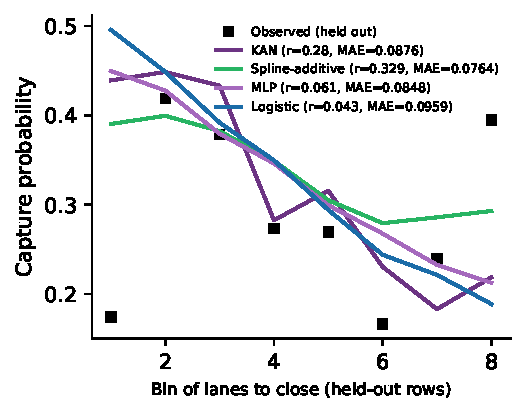
\includegraphics[width=0.6\textwidth]{F7_kan_mlp_logistic_shapes.pdf}
\caption{Observed held-out capture by bin of lanes to close, and the mean prediction of each model for the same rows
(matched estimand; DEVELOPMENT and TEST rows pooled; descriptive). Post hoc.}
\label{fig:s-kan}
\end{figure}

On TEST, the AUC is 0.597 for the KAN, against 0.645 (spline-additive), 0.647 (MLP) and 0.646 (logistic). The
observed KAN differences are about $-0.05$, with family 95\% intervals of roughly [$-$0.11, 0.01]. On DEVELOPMENT, AUCs
are 0.573, 0.575, 0.553 and 0.566, and every interval for a KAN difference includes zero. Bin-level correlations with
observed capture across lanes to close are, on TEST, 0.68, 0.80, 0.65 and 0.63, and on DEVELOPMENT, 0.28, 0.29, 0.10
and 0.02. The observed KAN minus spline-additive differences are $-0.12$ and $-0.01$, and all their intervals include
zero. No KAN advantage was detected, in line with controlled comparisons of KANs and MLPs \cite{yu2024kanfair}; this
does not establish equality. Pruning and symbolic distillation of the KAN give a near-linear logit dominated by lanes
to close: $-0.744$ per unit of the scaled feature, that is, $-0.186$ logit per additional lane. All four models
describe the same association. We do not claim a KAN-specific interpretability advantage. Two earlier analyses are
withdrawn: one compared partial-dependence curves with conditional means, which are different estimands, and one ran a
bootstrap that split true scenario families.

% =====================================================================================================
\section{Probes of the Inherent Limitations}\label{sec:s-probes}

Three limitations of the study cannot be removed: it is a simulation, its evaders are scripted, and its vehicles obey
SUMO's kinematics. Three registered probes test how much the main contrasts depend on them. None uses a TEST city.

\emph{Kinematic model.} On fresh scenarios of the seven development-phase cities (avoidant and random evaders, teams
of 3, 5 and 7, 20 scenarios and two SUMO seeds), PLB and pursuit were run under three variants with the same scenarios
and seeds: the model used throughout (Euler position update, Krau{\ss} car-following), a ballistic position update,
and IDM car-following. Of 10\,080 scheduled episodes, 252 failed scenario placement, in 42 conditions that fail
identically for both controllers and all variants (273 families per variant). A development check confirmed
beforehand that both options change the simulated trajectories. Both registered primaries were met
(Table~\ref{tab:s-probes}). OC rates under the two alternatives differ from the reference by at most 0.018, with
intervals that include zero. Eight episodes were flagged as collided, all from one scenario and seed and for both
controllers; none is a capture.

\emph{Background traffic.} Earlier in the project, background traffic had been tested only for the pursuit team. The
same scenarios and seeds were therefore run again with about 300 random-trip passenger cars per city (3\,360
scheduled episodes, 84 placement failures in the same 42 conditions). The reference without traffic is the first row
of Table~\ref{tab:s-probes}. The registered primary was met: with traffic, PLB minus pursuit is $+0.094$
[0.060, 0.130] (city~$\to$~family [0.050, 0.137]). Traffic lowers capture by PLB by $-0.062$ [$-$0.095, $-$0.030] and
by pursuit by $-0.029$ [$-$0.063, 0.004]. The advantage observed with traffic is 0.032 smaller than without; a post
hoc interval for that difference reaches zero ([$-$0.066, 0.000]; city~$\to$~family [$-$0.077, 0.012]), so a smaller
advantage with traffic is not established. PLB estimates arrival times in free flow, which could lower its capture
with traffic; this was not tested. The gap between the 5\,m rule and OC is
unchanged. The traffic is one level of random trips; it is not calibrated demand, and background drivers do not react
to the pursuit.

\begin{table}[!h]
\centering
\caption{PLB and pursuit under alternative kinematic models and with background traffic. Same scenarios and seeds in
every row. OC capture rates; family-clustered 95\% intervals.}
\label{tab:s-probes}
\begin{adjustbox}{max width=\textwidth}
\begin{tabular}{@{}lcccc@{}}
\toprule
Condition & PLB & Pursuit & PLB $-$ pursuit & Body gap 5\,m $-$ OC, pursuit \\
\midrule
Reference model & 0.439 & 0.313 & $+0.126$ [0.090, 0.164] & $+0.619$ [0.573, 0.665] \\
Ballistic position update & 0.443 & 0.303 & $+0.140$ [0.103, 0.177] & $+0.631$ [0.586, 0.676] \\
IDM car-following & 0.449 & 0.331 & $+0.118$ [0.079, 0.158] & $+0.581$ [0.531, 0.630] \\
Reference model, background traffic & 0.377 & 0.283 & $+0.094$ [0.060, 0.130] & $+0.638$ [0.593, 0.682] \\
\bottomrule
\end{tabular}
\end{adjustbox}
\end{table}

\emph{An evader tuned against PLB.} All other evaders are fixed scripts. This study gives the evader the kind of tuning
that PLB received. A new evader level scores every continuation by a weighted sum of seven features and takes the
best; a cul-de-sac ranks last while an alternative exists. The features use only the pursuers' current positions:
\begin{itemize}
\item the road distance from the end of the continuation to the nearest pursuer and to the second nearest, each
capped at 1\,000\,m;
\item the number of onward continuations, capped at four;
\item the share of pursuers within 300\,m of its end;
\item whether a pursuer is on the continuation or on one of its continuations;
\item whether it is the continuation that a distance-greedy predictor expects;
\item a reproducible random number.
\end{itemize}
With weight one on the first feature and zero elsewhere, the rule makes the same choice as the optimal evader, which
a unit test checks in 800 random states; this reference runs on the same scenarios as the tuned evader. The four
existing evader levels were re-run on 140 recorded episodes before and after the source change, with identical
outcomes.

The search used the TRAINING cities and one objective, the lowest OC capture by PLB. Thirty-two weight vectors were
drawn uniformly in $[-1,1]$ with a fixed seed. A first rung (four cities, six scenarios, team of five) kept the eight
best. A second rung (four cities, 20 scenarios, teams of 3, 5 and 7) selected one. Against the selected evader, PLB
captures 0.271 on the second rung, against 0.367 for the reference. The selected weights are $-0.87$ on the nearest
distance, $-0.89$ on occupied continuations and $+0.87$ on the random term, with the others between $-0.14$ and
$+0.27$: the evader avoids roads that carry a pursuer, is hard to predict, and does not seek distance.

The test used fresh scenarios on the seven development-phase cities (20 scenarios, two SUMO seeds, teams of 3, 5 and
7). Of 4\,200 scheduled episodes, 190 failed scenario placement, in 38 conditions that fail identically for all five
arms (134 families). Table~\ref{tab:s-tuned} gives the rates. The registered primary was met: PLB minus pursuit against
the tuned evader is $+0.128$ [0.081, 0.178] (city~$\to$~family [0.061, 0.198]), and $+0.097$, $+0.127$ and $+0.162$
for teams of 3, 5 and 7. Relative to the reference, the tuned evader changes capture by PLB by $-0.034$
[$-$0.099, 0.031] and by pursuit by $+0.010$ [$-$0.039, 0.059]. The reduction seen in the search (0.096) is therefore
mostly not reproduced on fresh scenarios. The family is scripted and small; a learned evader or a game-theoretic best
response could be stronger.

\begin{table}[!h]
\centering
\caption{OC capture against an evader tuned against PLB and against the reference (optimal) evader, on the same fresh
scenarios. Family-clustered 95\% intervals.}
\label{tab:s-tuned}
\begin{adjustbox}{max width=\textwidth}
\begin{tabular}{@{}lcccc@{}}
\toprule
Evader & PLB & Junction ambush & Pursuit & PLB $-$ pursuit \\
\midrule
Tuned against PLB & 0.29 & 0.25 & 0.16 & $+0.128$ [0.081, 0.178] \\
Reference (optimal) & 0.32 & -- & 0.15 & $+0.172$ [0.115, 0.232] \\
\bottomrule
\end{tabular}
\end{adjustbox}
\end{table}

% =====================================================================================================
\section{Reproducibility and Command Bookkeeping}\label{sec:s-repro}

\emph{Source recoverability.} Packages store source hashes rather than complete source snapshots. Seven dated
archives of the sources were taken during the audits. Of the 69 packages that recorded source hashes at launch, 14
are fully recoverable from those archives, including the studies added after the archives began, and 55 only in
part: for the earlier packages, later edits are documented by amendments, but some launch versions cannot be
recovered. The map is produced by a script and lists every recorded file. Replays with the historical behaviour reproduced every sealed outcome
we re-ran: 1\,433 captures, 600 sampled episodes, and 500 episodes sampled from five further packages.

\emph{Command bookkeeping.} Historical runs recorded orders that had no route, or that failed and fell back to a
default stop, as applied. The bookkeeping is corrected. Re-running the full PLB test cohort and the goal-directed
cohort with it (8\,966 episodes) changed no outcome and no contrast. In 58 of 58 re-runs compared in full, the
positions of all vehicles agreed to 1\,mm at every 0.1\,s step (speed, heading and lane were not compared). A
fallback remains an attempted manoeuvre whose exceptions are suppressed; logging it does not show that the manoeuvre
succeeded physically. Other historical cohorts were not re-run.

\emph{Invalid values.} The judge compared speeds without checking that they were finite, so a trace with a
non-finite speed could have been judged a capture. The judge now returns ``unknown'' for a trace that contains a
non-finite value, a negative speed or a non-positive body dimension, and such an episode is not counted as a
capture. For a trace without such values the verdict is unchanged. No such value was found in the 4.28 million
frames of the 1\,433 replayed captures or in the 512 reconstructed training episodes. Other historical traces were
not stored and could not be scanned.

\emph{Log files altered after sealing, and restored.} A simulator process that outlives its run keeps the run's log
file open. When such leftover processes received a termination signal, each wrote one line to the log of a package
that had already been sealed, in 14 packages. In every case the sealed content was intact as a prefix of the file
and the added bytes were only that line, repeated. The 14 files were cut back to their sealed length, which
restores their recorded checksums; the added bytes are kept, with a manifest. No result file was affected. Until
then a seal stated that every writer of the package had ended without checking it. The sealing tool now asks the
operating system whether any process holds a file of the package open for writing, refuses to seal if one does, and
records the check in the seal; the statement in earlier seals is the operator's declaration only. A check of all 89
sealed packages after the leftover processes were ended found no process holding any of their files.

% =====================================================================================================
\section{Registration, Addenda and Counting}\label{sec:s-ledger}

\emph{Counting.} The count is produced by a script with one explicit rule per package and block
(\path{scripts/count_episodes.py}); it replaces figures that earlier versions had assembled by hand. In our
setting the studies behind the article completed 197\,655 evaluation episodes, each run to estimate a rate or a
contrast that the article reports. A further 16\,403 episodes were used to select parameters or candidates (the
search rungs and search validation of PLB, of the seven-pursuer sensitivity study and of the tuned evader) and are
not evaluation data. A further 22\,455 runs were replays of earlier episodes for audits, and 6\,483 scheduled tasks
failed, almost all because the scenario generator could not place the team; such failures affect all methods of a
condition identically. Episodes generated while training a learner, validation during training and development
checks are not counted; the 499 training episodes replayed to audit the training loop are counted as replays. The
audits of the two published environments add 2\,484 episodes and 1\,709 replays in those environments. These are
counts of simulations. Episodes of one scenario family are not independent observations,
which is why every interval in the article resamples families.

\emph{Registered and post hoc analyses.} Table~\ref{tab:s-ledger} lists the studies behind the article and whether
their primary analysis was registered before the runs.

{\small
\setlength{\tabcolsep}{4pt}
\begin{longtable}{@{}>{\raggedright\arraybackslash}p{0.24\textwidth}>{\raggedright\arraybackslash}p{0.12\textwidth}>{\raggedright\arraybackslash}p{0.26\textwidth}>{\raggedright\arraybackslash}p{0.29\textwidth}@{}}
\caption{Studies behind the article. ``Registered'' means that the protocol and the primary analysis were recorded,
and sources hashed, before the runs. Outcomes are stated for the primary analysis.}
\label{tab:s-ledger}\\
\toprule
Study & Registered & Primary analysis & Outcome \\
\midrule
\endfirsthead
\toprule
Study & Registered & Primary analysis & Outcome \\
\midrule
\endhead
\bottomrule
\endfoot
Endpoint robustness (three evaders, team sizes, grids) & yes & team minus independence reference & no supported excess in 10 cells \\
Junction ambush & yes & ambush minus pursuit & $+0.04$ to $+0.12$ \\
Option PPO (MLP, KAN) & yes & learned minus rule & $0.000$ [$-$0.004, 0.004] \\
PLB parameter search and test & yes & PLB minus junction ambush & $+0.050$, met \\
Oracle evader model & no & descriptive & $+0.03$ to $+0.04$, intervals include zero \\
Pursuer speed & no & descriptive & $-0.07$ to $+0.03$ \\
First MAPPO study (first implementation) & yes & MAPPO minus planner & met on its own test ($+0.047$ MLP, $+0.052$ KAN); see Table~\ref{tab:s-imitation} \\
Decision-commitment replication & yes & 3\,s minus 1\,s commitment & $+0.010$ [$-$0.012, 0.033], not confirmed \\
Hold audit of OC & yes & escapes with pursuers held & 0 of 1\,433 after follow-up completion \\
Held-out evaluation (TEST) & yes & PLB minus pursuit; proximity minus OC & both met \\
Goal-directed evader & yes & PLB minus pursuit & $+0.105$, met \\
MAPPO-v2 (first implementation) & yes & v2 minus PLB & not met; fine-tuning affected by an implementation defect \\
Coordination ablation & yes & coordinated minus independent PLB & $+0.071$, met \\
Active-escape probe & yes & descriptive & 15 of 1\,433 escapes \\
Null team; joint escape; clustered intervals & yes (as corrections) & descriptive & see article \\
Proximity-trained MAPPO (first implementation) & yes & widening of the gap between endpoints & $+0.170$, met; not reproduced after correction (see MAPPO-v3) \\
MAPPO-v3 (corrected controller) & yes & validated gain on imitation; widening of the gap under proximity training & neither met; the earlier decline did not recur; training loop later found defective \\
Second published environment (PEPCRL-MVP) & yes & descriptive, with a registered prediction & no same-lane capture in 2\,380 events; prediction held \\
Second held-out set (HELD-OUT~B) & yes & PLB minus pursuit; proximity minus OC & both met ($+0.064$; $+0.549$) \\
Comparison of the two held-out sets & no & post hoc & advantage of PLB smaller on the second set \\
Capture instants of the hold audit, re-verified & yes (as correction) & descriptive & 1\,433 of 1\,433 confirmed; none affected \\
First training batches of MAPPO-v3, reconstructed & yes (as correction) & descriptive & 8 of 8 batches reproduced; 0.6\% of trained decisions had no future \\
MAPPO-v4 (corrected training loop) & yes & validated gain on imitation; widening of the gap under proximity training & neither met; conclusions of MAPPO-v3 unchanged \\
Published environment, addendum & yes (as correction) & descriptive & 12 of 12 follow-ups and 800 of 800 re-runs reproduce the original events \\
Published environment (DGMARL-MVP) & yes & descriptive & no same-lane capture in 999 events \\
Kinematic model (ballistic update; IDM) & yes & PLB minus pursuit under each & $+0.140$ and $+0.118$, both met \\
Background traffic & yes & PLB minus pursuit with traffic & $+0.094$, met \\
Evader tuned against PLB & yes & PLB minus pursuit against it & $+0.128$, met \\
KAN, spline, MLP, logistic models & no & post hoc & no KAN advantage detected \\
Lane-duplication diagnostics & no & post hoc & 49\% versus 0\% duplicated targets \\
\end{longtable}
}

The first MAPPO study met its primary on its own test set, with a gain over the planner of about 0.05. Later results
are mixed (Table~\ref{tab:s-imitation}): on the held-out cities the same controllers show no detected difference from
PLB, the MAPPO-v2 study did not meet its primary, a post hoc contrast on a further test set is again positive, and
the MAPPO-v3 and MAPPO-v4 test sets give differences whose intervals include zero. A registered replication of one suspected cause, a 3\,s decision commitment, was not confirmed. In every
study the retained controllers are imitation checkpoints, so the article attributes no gain to reinforcement learning
and leaves the cause of the small difference open.
Earlier phases of the project (constructive caging certificates and reinforcement-learning pilots with a gate
heuristic), closed before the studies above, are not used in the article; their records are part of the repository.

\emph{Versioned corrections.} Six addenda corrected earlier analyses without relabelling original outputs:
\begin{itemize}
\item \emph{Addendum 1} completed the 60\,s follow-up of 188 censored hold-audit replays, introduced joint escape
(gate or network exit) for the containment indicators, and replaced cell-level bootstraps by family-clustered and
city~$\to$~family bootstraps. The article reports the pre-registered cell interval of the held-out primary together
with the corrected ones.
\item \emph{Addendum 2} verified each extended replay against its original capture, added family intervals for the
null team and the indicators, recomputed the KAN comparison with true scenario families, and corrected the command
bookkeeping.
\item \emph{Addendum 3} added the coordination ablation, the active-escape probe and the large-scale re-runs with the
corrected bookkeeping. One runner of this addendum was changed during the run to add a stall timeout; the change is
documented in the package and does not alter any episode.
\item \emph{Addendum 4} followed a fourth audit. It completed the follow-up of 12 censored cases in the
published-environment audit and replaced its stop analogue by one with a duration measured in simulation time
(Section~\ref{sec:s-published}); it identified the implementation defect of the learning studies and repeated them
with a corrected controller (Section~\ref{sec:s-learning}); and it added a post hoc interval for the effect of
traffic on the advantage of PLB.
\item \emph{Addendum 5} followed a fifth audit. It replayed the 1\,433 audited captures to verify each capture instant
with a corrected extractor (Section~\ref{sec:s-hold}); it made the judge reject invalid values
(Section~\ref{sec:s-repro}); it corrected the training loop and measured the incidence of its two defects on the
first training batch of every MAPPO-v3 run, and then repeated the learning block with the corrected loop
(Section~\ref{sec:s-learning}); it withdrew the attribution of the earlier decline under fine-tuning to one defect; it recorded an arithmetic erratum of a registered protocol; and it added
an antecedent that the article had omitted \cite{bykov2025interceptor}.
\item \emph{Addendum 6} followed a sixth audit and ran no simulation. It stated the denominators of the second
published environment, with the 22 capture events recorded before an abort (Section~\ref{sec:s-published}); it made
the sealing tool check that no process still writes to a package (Section~\ref{sec:s-repro}); it replaced ``no
deterioration'' by a wording that does not suggest a demonstrated equivalence and separated training attempts from
valid episodes (Section~\ref{sec:s-learning}); and, after the full text of \cite{bykov2025interceptor} had been
read, it corrected the description of that study in the article.
\end{itemize}

\bibliographystyle{elsarticle-num}
\bibliography{refs}

\end{document}
